\documentclass[a4paper,12pt]{article} % Тип документа



\usepackage{graphicx}
\graphicspath{{pictures/}}
\DeclareGraphicsExtensions{.pdf,.png,.jpg}
\usepackage{multirow}

% Русский язык
\usepackage[T2A]{fontenc}
\usepackage[utf8]{inputenc}
\usepackage[english,russian]{babel}

% Математика
\usepackage{amsmath,amsfonts,amssymb,amsthm,mathtools} 


\usepackage{wasysym}

%Заговолок
\author{Маллаев Руслан}
\title{Лабораторная работа №3.2.4 \\ Свободные колебания в электрическом контуре}
\date{09 сентября 2021 г.}

\begin{document} % Начало документа

\maketitle
\newpage
 
 \textbf{Цель работы:} Исследование свободных колебаний в электрическом контуре.\\

\textbf{Приборы, используемые в работе:} Генератор импульсов, электронное реле, магазин сопротивлений, магазин емкостей, катушка индуктивности, электронный осциллограф, универсальный измерительный мост.

\section*{Теория}
\subsection*{Свободные колебания}
Рассмотрим электрический контур, состоящий из последовательно соединённых конденстора $C$, катушки индуктивности $L$ и резистора $R$. Обозначим разность потенциалов на конденсаторе $U_C$, а ток, текущий в контуре, через $I$. Второе првило Кирхгофа:
\begin{equation}
L \dfrac{d^2I}{dt^2}+R\dfrac{dI}{dt}+\dfrac{I}{C}=0.
\end{equation}
Вводя обозначения $\gamma = \dfrac{R}{2L}$, $\omega_0^2=\dfrac{1}{LC}$, получим уравнение
\begin{equation}
\ddot{I}+2\gamma\dot{I}+\omega_0^2I=0.
\end{equation}
Его решение в общем виде:
\begin{equation}
I = -\dfrac{U_0}{L\kappa}e^{-\gamma t}\text{sh}(\kappa t), 
\end{equation}
где $\kappa = \sqrt{\gamma^2 - \omega_0^2}$, $U_0 = U_C$ -- начальное напряжение на конденсаторе.

\subsection*{Затухающие колебания}
 В случае, когда $\gamma < \omega_0$, имеем $\kappa = i\omega$, где $\omega = \sqrt{\omega_0^2 - \gamma^2}$ -- \textit{частоты свободных (собственных) колебаний}. Тогда ток
 \begin{equation}
 I = -\dfrac{U_0}{L\omega}e^{-\gamma t}\sin(\omega t)
 \end{equation}
 затухает и имеет колебательный характер. Величина $\gamma$ определяет затухание колебаний: $\gamma = \dfrac{1}{\tau}$, где $\tau$ -- время затухание амплитуды в $e$ раз.
Формулы для наряжение на кондесаторе и тока в цепи можно переписать иначе:
\begin{equation}
\begin{array}{c}
U_C = U_0 \dfrac{\omega_0}{\omega}e^{-\gamma t} \cos(\omega t - \theta),\\
\\
I = -\dfrac{U_0}{L}e^{-\gamma t} \cos(\omega t - \theta).
\end{array}
\end{equation}
\subsection*{Апериодические колебания}
В случае $\gamma > \omega_0$, формулы для тока и напряжения на конденсаторе имеют следующий вид:
$$
\begin{array}{c}
I = -\dfrac{U_0}{L\kappa}e^{-\gamma t}\text{sh}(\kappa t),\\
\\
U_C = U_0 e^{-\gamma t}\left( \dfrac{\gamma}{\kappa}\text{sh}(\kappa t) + \text{ch}(\kappa t) \right).
\end{array}
$$
Процесс в этом случае не является колебательным, его называют апериодическим. Режим, соответствующий $\gamma = \omega_0$, называются \textit{критическим}. В этом случае предельный переход $\omega \rightarrow 0$ в $(5)$ даст 
$$
\begin{array}{c}
I = -\dfrac{U_0}{L}te^{-\gamma t},\\
\\
U_C=U_0 e^{-\gamma t}(1+\gamma t).
\end{array}
$$
Сопротивление в этом случае 
\begin{equation}
R_{\text{кр}}= 2 \sqrt{\dfrac{L}{C}}
\end{equation}
называется \textit{критическим сопротивлением} контура.\\
\textit{Добротность} контура по определению 
$$
Q = 2\pi \dfrac{W}{\Delta W},
$$ 
где $W$ -- запасённая энергия, $\Delta W$ -- потери за период. Тогда
$$
Q = 2\pi\dfrac{CU_0^2/2 \cdot e^{-2\gamma t}}{CU_0^2/2 \cdot (e^{-2\gamma t} - e^{-2\gamma (T+t)})}=\dfrac{\pi}{\gamma T}=\dfrac{1}{R}\sqrt{\dfrac{L}{C}}.
$$
\textit{Логарифмическим декрементом затухания} называются число
$$
\Theta = \text{ln}\dfrac{U_k}{U_{k+1}}=\text{ln} e^{\gamma T}=\gamma T
$$
или 
$$
\Theta = \dfrac{1}{n} \text{ln}\dfrac{U_k}{U_{k+n}}.
$$
\newpage
\section*{Установка}
\begin{figure}[h!]
\begin{center}
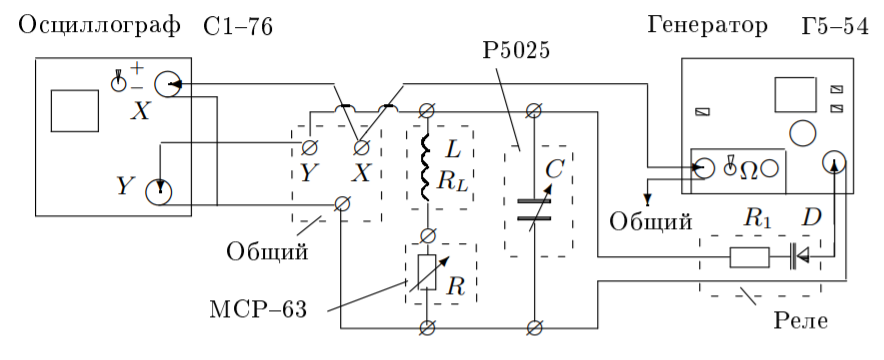
\includegraphics[width = 0.7\textwidth]{1.png}
\caption{Схема установки}
\end{center}
\end{figure}
На рисунке приведена схема для исследования свободных колебаний в контуре, содержащем постоянную индуктивность $L$ и переменные ёмкость $C$ и сопротивление $R$. Колебания наблюдаются на экране осциллографа.

Для периодического возбуждения колебаний в контуре используется генератор импульсов Г5-54. С выхода генератора по коаксиальному кабелю импульсы поступают на колебательный контур через электронное реле, смонтированное в отдельном блоке (или на выходе генератора). Реле содержит тиристор $D$ и ограничительный резистор $R_1$.

Импульсы заряжают конденсатор $C$. После каждого импульса генератор отключается от колебательного контура, и в контуре возникают свободные затухающие колебания. Входное сопротивление осциллографа велико ($\approx 1$ МОм), так что его влиянием на контур можно пренебречь. Для получения устойчивой картины затухающих колебаний используется режим ждущей развёртки с синхронизацией внешними импульсами, поступающими с выхода <<синхроимпульсы>> генератора.
\newpage
\section*{Ход работы}
Прежде всего измерим индуктивность $L$ и сопротивление катушки $R_L$ в зависимости от частоты 

\begin{table}[h!]
\begin{center}

\begin{tabular}{|c|c|c|}
\hline
$\nu$, Гц & $L$, мГн & $R_L$, Ом \\ \hline
50        & 146.1    & 11.71      \\ \hline
1000      & 140.2    & -0.72      \\ \hline
5000      & 142.0    & -33.6      \\ \hline
\end{tabular}
\caption{Некоторые параметры катушки индуктивности}
\end{center}
\end{table}
В итоге мы получаем, что $L = (143.0 \pm 1.6)$ мГн. 
\subsection*{Измерение периодов свободных колебаний}
Установим на магазине сопротивлений $R = 0$ Ом и $C = 0,02$ мкФ. Подобрав частоту развертки получим изображение наших колебаний на осциллографе. Из этого убедимся, что частота повторений, которую мы установили на генераторе ($\nu_0 = 100$ Гц) будет равна частоте повторения импульсов. 

\begin{figure}[h!]
\begin{center}
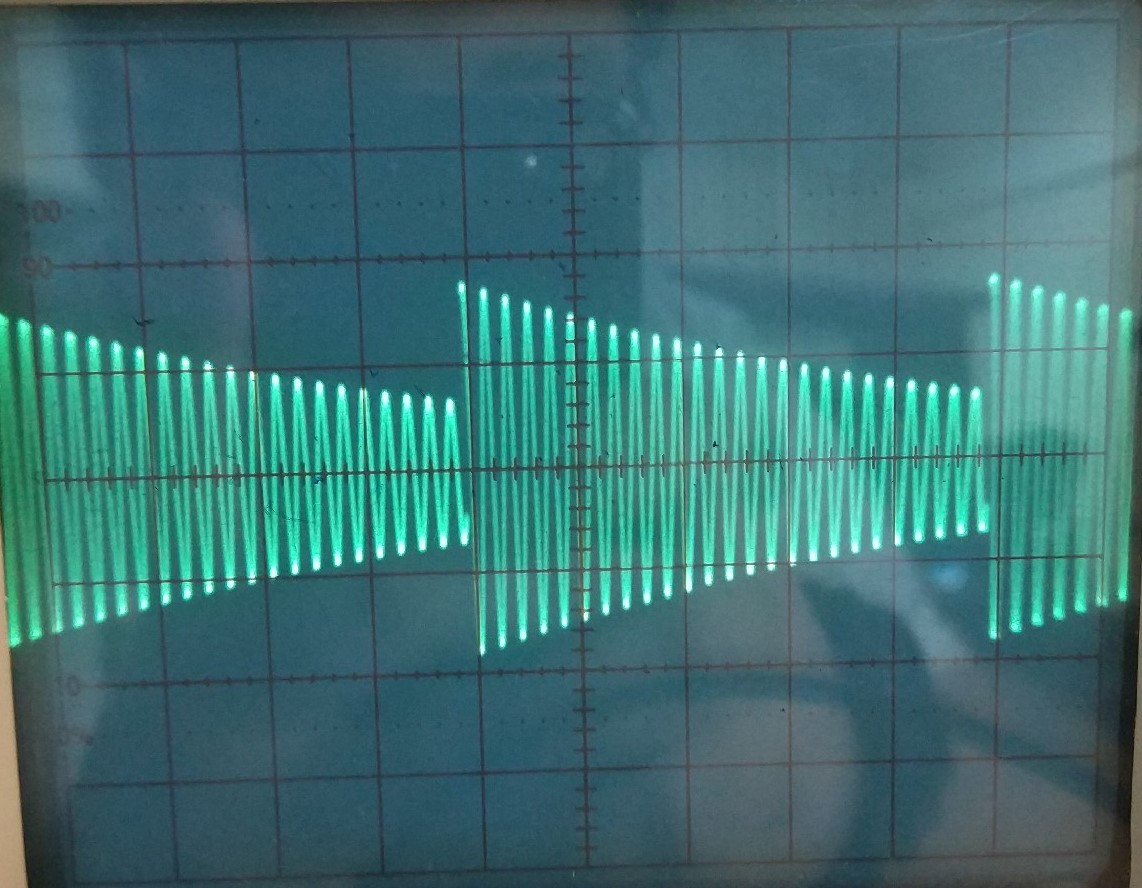
\includegraphics[width = 0.5\textwidth]{3.jpg}
\caption{Колебания в контуре}
\end{center}
\end{figure}

Теперь изменяя ёмкость в диапазоне $0,02 - 0,9$ мкФ проведем измерения периодов свободных колебаний и сравним их с теоретическими данными по формуле 
\[T = 2 \pi \sqrt{LC}\]

\begin{table}[]
\begin{center}
\begin{tabular}{|c|c|c|c|c|c|c|}
\hline
C, нФ & t, мс & $\sigma_t$, мс & N периодов & $T_{exp}$, мс & $T_{theor}$, мс & $\sigma_T$, мс \\ \hline
20    & 9.6   & 0.2   & 28.0       & 0.34  & 0.33  & 0.01  \\ \hline
25    & 9.6   & 0.2   & 25.0       & 0.38  & 0.37  & 0.01  \\ \hline
30    & 9.6   & 0.2   & 23.0       & 0.42  & 0.41  & 0.01  \\ \hline
40    & 9.6   & 0.2   & 20.0       & 0.48  & 0.47  & 0.01  \\ \hline
50    & 9.6   & 0.2   & 18.0       & 0.53  & 0.53  & 0.01  \\ \hline
60    & 9.6   & 0.2   & 17.0       & 0.56  & 0.58  & 0.01  \\ \hline
70    & 9.6   & 0.2   & 15.0       & 0.64  & 0.63  & 0.01  \\ \hline
90    & 9.6   & 0.2   & 13.0       & 0.74  & 0.71  & 0.02  \\ \hline
150   & 9.6   & 0.2   & 10.0       & 0.96  & 0.92  & 0.02  \\ \hline
200   & 9.6   & 0.2   & 9.0        & 1.07  & 1.06  & 0.02  \\ \hline
300   & 9.6   & 0.2   & 7.0        & 1.37  & 1.30  & 0.03  \\ \hline
400   & 9.6   & 0.2   & 6.0        & 1.6   & 1.50  & 0.03  \\ \hline
500   & 9.6   & 0.2   & 5.5        & 1.75  & 1.67  & 0.04  \\ \hline
700   & 9.6   & 0.2   & 5.0        & 1.92  & 1.98  & 0.04  \\ \hline
900   & 9.6   & 0.2   & 4.5        & 2.13  & 2.25  & 0.04  \\ \hline
\end{tabular}
\end{center}
\end{table}

Построим график, чтобы оценить сходство эксперимента с теорией.\\
\begin{figure}[h!]
\begin{center}
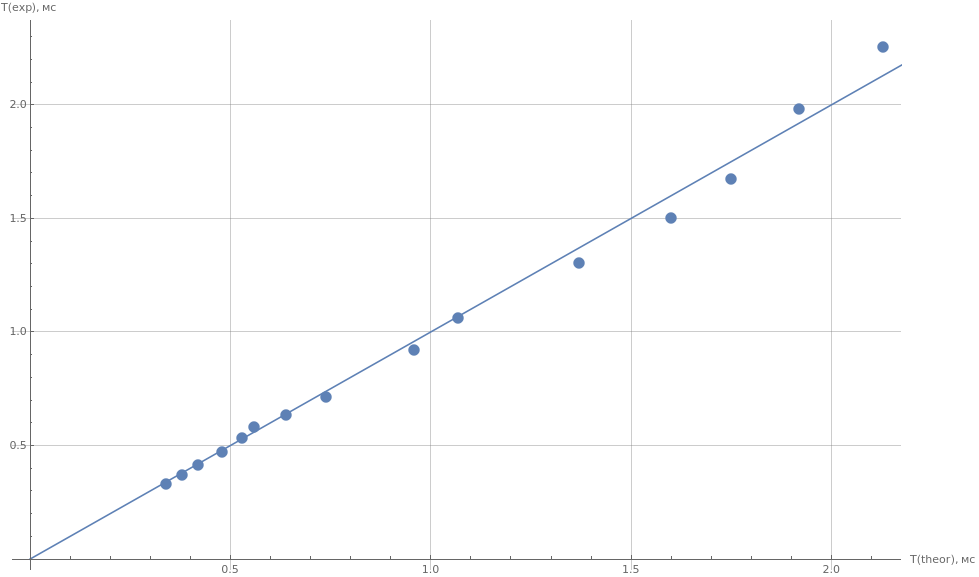
\includegraphics[width = 0.9\textwidth]{2.png}
\caption{Зависимость $T_{exp}$ от $T_{theor}$}
\end{center}
\end{figure}\\
По графику видно, что эксперимент согласуется с теорией.
\newpage
\section*{Измерение критического сопротивления и декремента затухания}
Для начала рассчитаем емкость, при которой частота собственных колебаний контура будет равна $\nu_0 = 5$ кГц.
\[C = \dfrac{1}{4 \pi^2 \nu_0^2 L} \approx 5 \text{нФ}\]
И для значений $L$ и $C$ рассчитаем $R_{crit}$
\[R_{crit} = 2\pi\sqrt{\dfrac{L}{C}} \approx 12,6 \text{кОм}\]
Для этих значений $L$ и $C$ рассчитаем декремент затухания для каждого сопротивления из интервала $(0,1-0,3)R_{crit}$. Из этих данных по формуле 
\[\theta = \frac{1}{n}\cdot\ln\frac{U_k}{U_{k+n}}\]
находим $\theta$ и запишем все в таблицу.
\[R_{\Sigma} = R_L + R\]
\\
 
\begin{table}[h]
\begin{center}
\begin{tabular}{|c|c|c|c|c|c|c|c|c|}
\hline
R, кОм & $U_1$, дел & $\sigma_{U_1}$, дел   & $U_{1 + n}$, дел & $\sigma_{U_{1 + n}}$, дел  & n & $\theta$ & $\sigma_{\theta}$ & $R_{\Sigma}$, кОм   \\ \hline
1.06   & 11.5    & 0.5 & 3.0     & 0.5 & 3 & 0.67  & 0.12 & 1.07\\ \hline
1.16   & 11.5    & 0.5 & 6.0     & 0.5 & 2 & 0.65  & 0.06 & 1.17\\ \hline
1.26   & 11.5    & 0.5 & 2.5     & 0.5 & 3 & 0.76  & 0.15 & 1.27\\ \hline
1.46   & 11.5    & 0.5 & 5.0     & 0.5 & 2 & 0.83  & 0.09 & 1.46\\ \hline
1.56   & 11.5    & 0.5 & 2.0     & 0.5 & 3 & 0.87  & 0.22 & 1.56\\ \hline
1.76   & 11.5    & 0.5 & 4.0     & 0.5 & 2 & 1.06  & 0.14 & 1.76\\ \hline
2.06   & 11.5    & 0.5 & 3.0     & 0.5 & 2 & 1.34  & 0.23 & 2.07\\ \hline
2.66   & 11.5    & 0.5 & 2.0     & 0.5 & 2 & 1.75  & 0.44 & 2.67\\ \hline
\end{tabular}
\end{center}
\end{table}

Для расчета $R_{crit}$ построим график $1/\theta^2 = f(1/R^2_{\Sigma})$. Приняв обозначение $1/\theta^2 = Y$ и $1/R^2_{\Sigma} = X$, можно показать, что $R_{crit} = 2\pi\sqrt{\Delta Y/\Delta X}$.
\newpage
\begin{figure}[h!]
\begin{center}
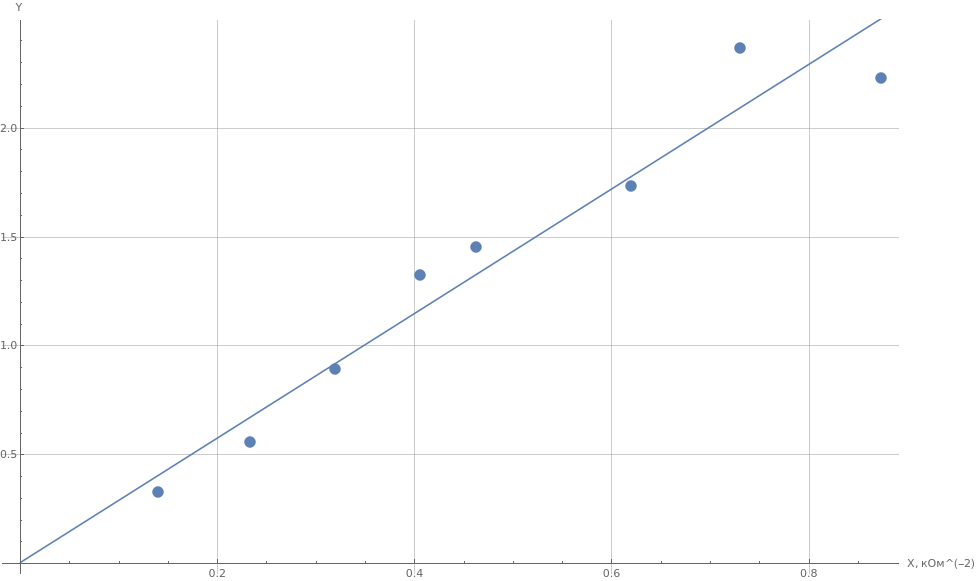
\includegraphics[width = 0.8\linewidth]{3.png}
\caption{Зависимость $1/\theta^2$ от $1/R^2_{\Sigma}$}
\end{center}
\end{figure}
А также выведем все коэффициенты, полученные при построении графика.\\
\begin{table}[h!]
\begin{center}
\begin{tabular}{|c|c|c|c|c|}
\hline
  & Estimate & Standard Error & t-Statistic & P-Value \\ \hline
1 & 0.006    & 0.149          & 0.040       & 0.969   \\ \hline
x & 2.859    & 0.282          & 10.138      & 0.000   \\ \hline
\end{tabular}
\end{center}
\end{table}\\
Из вышепредставленных коэффициентов получаем, $R_{crit} = (10.62 \pm 1.05)$кОм, что достаточно близко к теоретически рассчитанному значению.\\
Еще можно вычислить $R_{crit}$, подводя график к данному виду:\\
\begin{figure}[h!]
\begin{center}
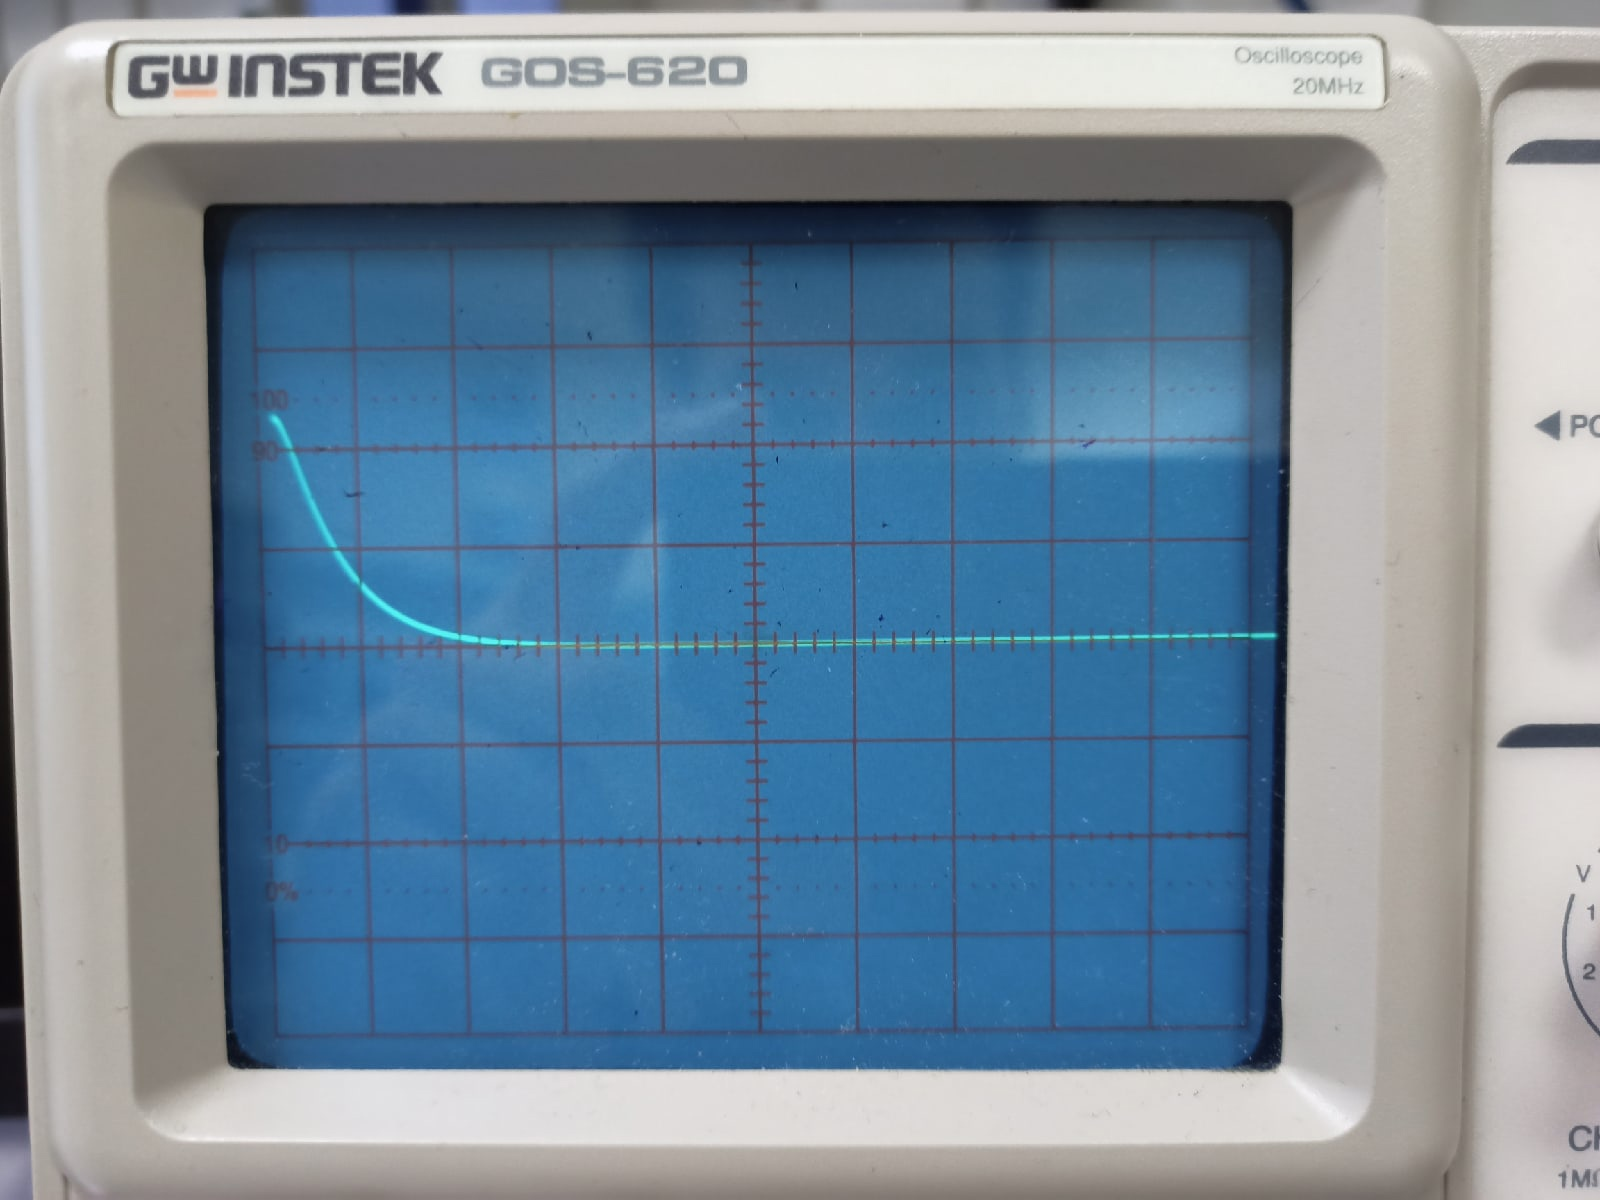
\includegraphics[width = 0.45\linewidth]{1.jpg}
\end{center}
\end{figure}\\
и фиксируя значение сопротивления: $R_{crit} = 12.5$ кОм.

\newpage
\subsection*{Свободные колебания на фазовой плоскости}
Рассмотрим свободные колебания на фазовой плоскости, для этого подключим место соединения катушки индуктивности и магазина сопротивлений к выходу $X$ и включим на осциллографе канал $X-Y$. В итоге мы получаем картинку на экране как на рисунке ниже. 
\begin{figure}[h!]
\begin{center}
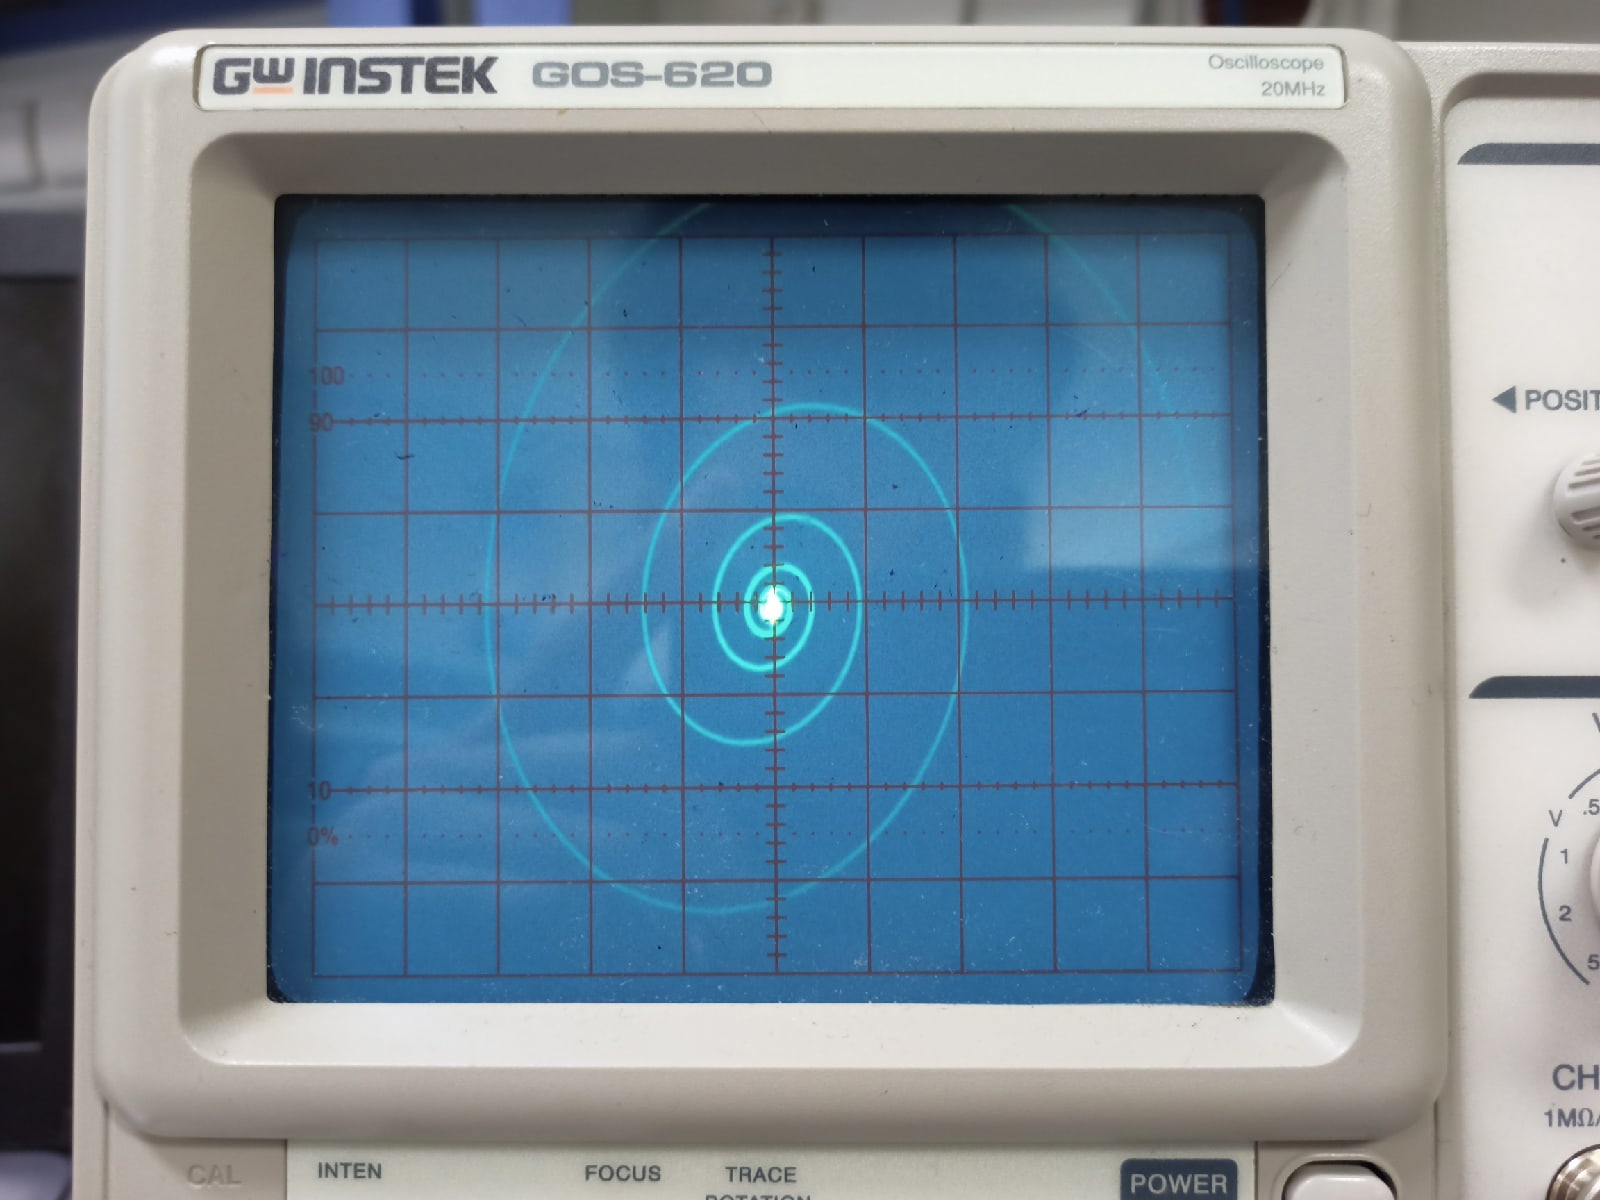
\includegraphics[width = 0.6\textwidth]{2.jpg}
\caption{Фазовая диаграмма для свободных колебаний}
\end{center}
\end{figure}

Для фазовой диаграммы для двух значений посчитаем так же декремент затухания
\\
\begin{table}[h!]
\begin{center}
\begin{tabular}{|c|c|c|c|c|c|c|}
\hline
R, кОм & $U_k$, дел & $U_n$, дел & n & k & $\theta$ & $\sigma_{\theta}$    \\ \hline
1.00   & 3.0     & 20.0    & 5 & 2 & 0.63  & 0.11 \\ \hline
1.26   & 2.0     & 5.0     & 3 & 2 & 0.91  & 0.24 \\ \hline
1.56   & 4.0     & 10.5    & 4 & 3 & 0.97  & 0.13 \\ \hline
2.00   & 2.5     & 10.0    & 3 & 2 & 1.39  & 0.28 \\ \hline
2.50   & 1.5     & 8.0     & 3 & 2 & 1.67  & 0.56 \\ \hline
\end{tabular}
\end{center}
\end{table}

Видим, что декремент затухания подсчитанный в предыдущей секции совпадает с декрементом затухания, полученным из фазовой диаграммы.
\newpage
\subsection*{Добротность свободных колебаний в контуре}
Добротность можно найти по формуле 
\[Q = \dfrac{\pi}{\theta}\]
Найдем ее для $R_{max} = 1$ кОм и для $R_{min} = 2.6$ кОм из графика и фазовой диаграммы. Итоговые результаты запишем в таблицу.

Так же добротность можно найти и из теоретических соображений по формуле
\[Q = \dfrac{1}{R}\sqrt{\dfrac{L}{C}}\]

Результаты так же занесем в таблицу, и в итоге мы получаем эту таблицу со всеми данными из данного эксперимента, по которой мы можем сравнить все полученные значения

\begin{table}[h!]
\begin{center}
\begin{tabular}{|c|c|c|c|c|c|c|c|}
\hline
\multirow{2}{*}{} & \multirow{2}{*}{$L_{coil}$, мГн} & \multicolumn{3}{c|}{$R_{crit}$, кОм}                         & \multicolumn{3}{c|}{Q}                 \\ \cline{3-8} 
                  &                                  & Теор.                 & Подбор              & Граф.          & Теор. & Граф.         & Спираль        \\ \hline
$R_{max}$         & \multirow{2}{*}{$143.0 \pm 1.6$}   & \multirow{2}{*}{12.6} & \multirow{2}{*}{12.5} & $10.62 \pm 1.05$ & 5.35   & $4.83 \pm 0.74$ & $4.99 \pm 0.87$  \\ \cline{1-1} \cline{5-8} 
$R_{min}$         &                                  &                       &                     & $10.62 \pm 1.05$ & 2.01   & $1.80 \pm 0.45$ & $1.88 \pm 0.63$ \\ \hline
\end{tabular}
\caption{Итоговые результаты эксперимента}
\end{center}
\end{table}
\section*{Вывод}
Как видно из таблицы 2, наилучший способ измерения добротности --- с помощью графика, потому что получаются наиболее близкие значения с меньшими погрешностями. Так же из графика видно, что $R_{crit}$ лучше измеряется при более высоком сопротивлении в контуре. 

\end{document}